\section{Dika Sukma Pradana(1174050)}
\subsection{Point Polyline dan Polygon}
\begin{enumerate}
	\item 
	\lstinputlisting{src/1/1174050/1.py}
	\begin{figure}[H]
		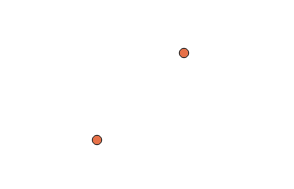
\includegraphics[width=12cm]{figures/1174050/1.PNG}
		\centering
		\caption{Point}
	\end{figure}
	
	\item 
	\lstinputlisting{src/1/1174050/2.py}
	\begin{figure}[H]
		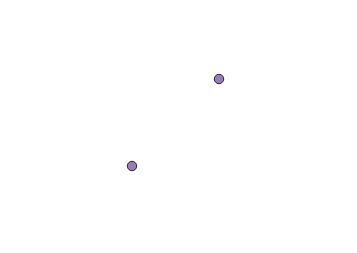
\includegraphics[width=12cm]{figures/1174050/2.PNG}
		\centering
		\caption{Point}
	\end{figure}
	
	\item 
	\lstinputlisting{src/1/1174050/3.py}
	\begin{figure}[H]
		
\includegraphics[width=12cm]{figures/1174050/3.PNG}
		\centering
		\caption{Point}
	\end{figure}
	
	\item 
	\lstinputlisting{src/1/1174050/4.py}
	\begin{figure}[H]
		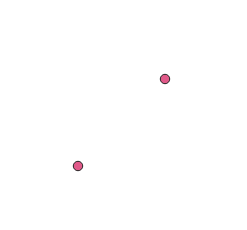
\includegraphics[width=12cm]{figures/1174050/4.PNG}
		\centering
		\caption{Point}
	\end{figure}
	
	\item 
	\lstinputlisting{src/1/1174050/5.py}
	\begin{figure}[H]
		
\includegraphics[width=12cm]{figures/1174050/5.PNG}
		\centering
		\caption{Polyline}
	\end{figure}
	
	\item 
	\lstinputlisting{src/1/1174050/6.py}
	\begin{figure}[H]
		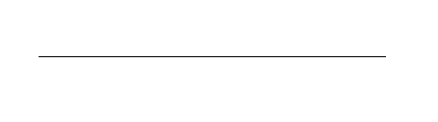
\includegraphics[width=12cm]{figures/1174050/6.PNG}
		\centering
		\caption{Poligon}
	\end{figure}
	
	\item 
	\lstinputlisting{src/1/1174050/7.py}
	\begin{figure}[H]
		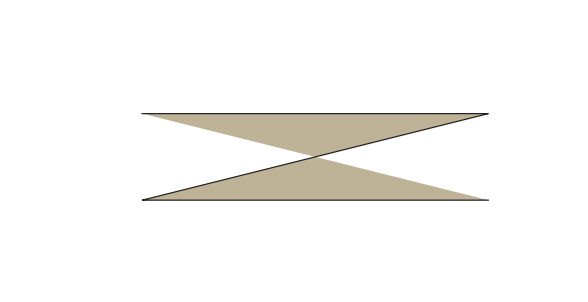
\includegraphics[width=12cm]{figures/1174050/7.PNG}
		\centering
		\caption{Polygon}
	\end{figure}
	
	\item 
	\lstinputlisting{src/1/1174050/8.py}
	\begin{figure}[H]
		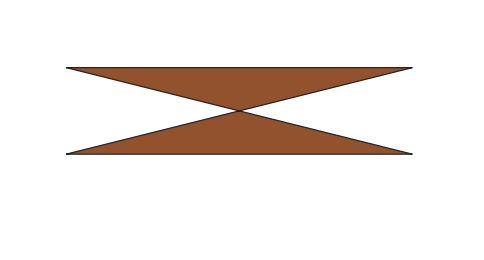
\includegraphics[width=12cm]{figures/1174050/8.PNG}
		\centering
		\caption{Polygon}
	\end{figure}
	
	\item 
	\lstinputlisting{src/1/1174050/9.py}
	\begin{figure}[H]
		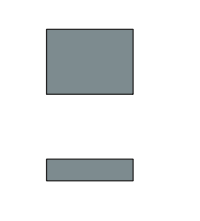
\includegraphics[width=12cm]{figures/1174050/9.PNG}
		\centering
		\caption{Polygon}
	\end{figure}
	
	\item 
	\lstinputlisting{src/1/1174050/10.py}
	\begin{figure}[H]
		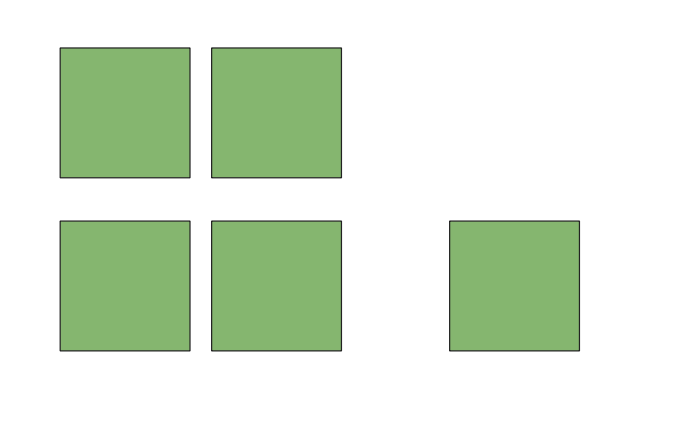
\includegraphics[width=12cm]{figures/1174050/10.PNG}
		\centering
		\caption{Hasil mod saya yaitu 2 jadi yang saya kerjakan Bujursangkar yang berjumlah 5, Polygon}
	\end{figure}	
\end{enumerate}

\subsection{Link}
\href{https://youtu.be/5X5gnr74VV4}{Youtube! JANGAN LUPA SESKREB!!}